% Chapter 2

\chapter{Method} % Write in your own chapter title
\label{Chapter:Method}
\lhead{Chapter 2. \emph{\steel}} % Write in your own chapter title to set the page header

\section{Why do we need a new modeling technique in galactic astrophysics.}
%What is missing: Massive galaxies, checks 
%How can a new model succeed where others haven't
\section{Designing to specification.}
%General format: Science problem and design solution 
%Volume/resolution - statistical
%Flexibility - empirical
%Consistency - ensuring connections between high and low redshift
%Systematics - speed
\section{Modules and Methods}
%Statistical Dark matter accretion history
\begin{figure}[h]
	\centering
	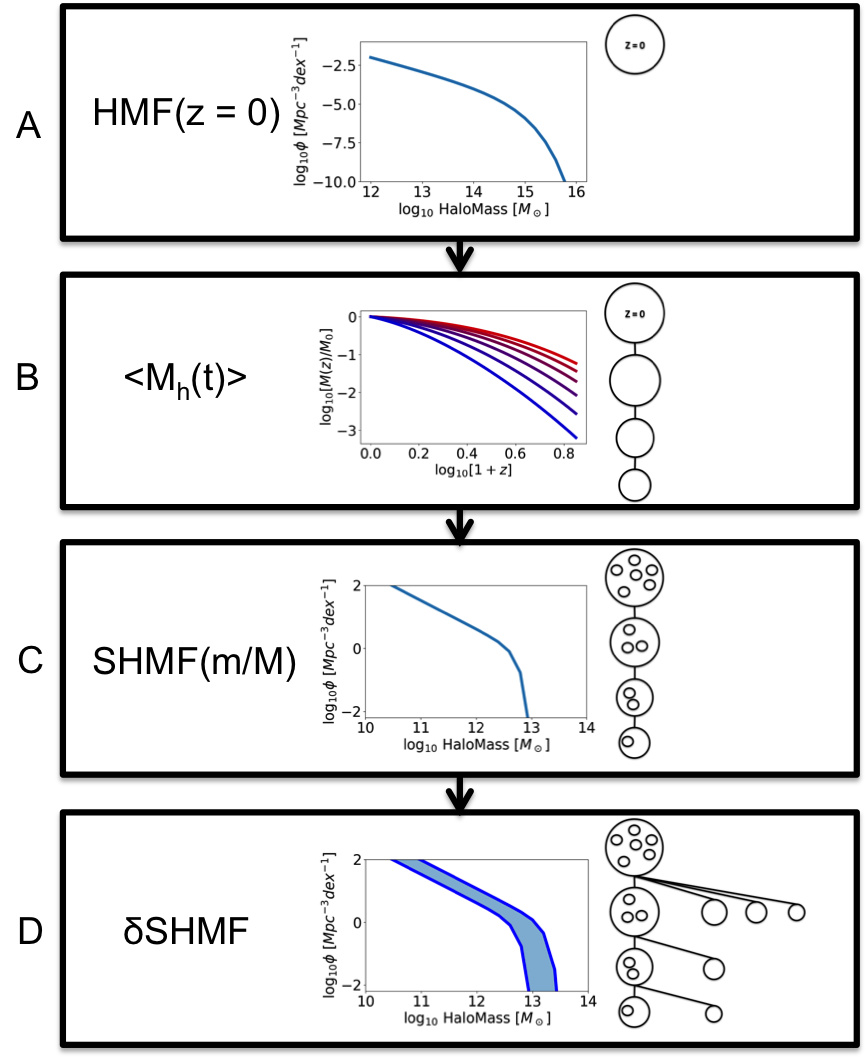
\includegraphics[width = \linewidth]{Figures/Chapter2/StatDM.png}
    \caption{We show the main steps in building the statistical dark matter accretion history for STEEL. Each panel shows a feature from a traditional merger tree and the statistical function used to replace it. A: The HMF is used to calculate the number densities of central haloes. B: Average mass growth histories are used to calculate the size of each mass bin at previous epochs. C: The (unevolved)SHMF is used to populate each central at each redshift with subhaloes. D: The average number densities of accreted subhaloes at each epoch, are calculated by taking the difference between each mass bin of the (unevolved)SHMF at consecutive redshift steps.}
	\label{fig:StatDM}
\end{figure}
%Abundace matching



%Continuity equation
%Mass recycling
%Central Postprocessing 
